\documentclass[tikz,border=4pt]{standalone}
\usepackage[T1]{fontenc}
\usepackage[utf8]{inputenc}
\usepackage{FiraSans}
\usepackage{amsmath}
\usetikzlibrary{arrows.meta,positioning,calc}
\definecolor{ceBlue}{RGB}{42,96,153}
\definecolor{ceTeal}{RGB}{36,135,118}
\definecolor{ceGold}{RGB}{220,160,52}
\definecolor{ceRed}{RGB}{188,74,60}
\definecolor{ceInk}{RGB}{42,42,42}
\definecolor{ceGray}{RGB}{238,240,242}
\begin{document}
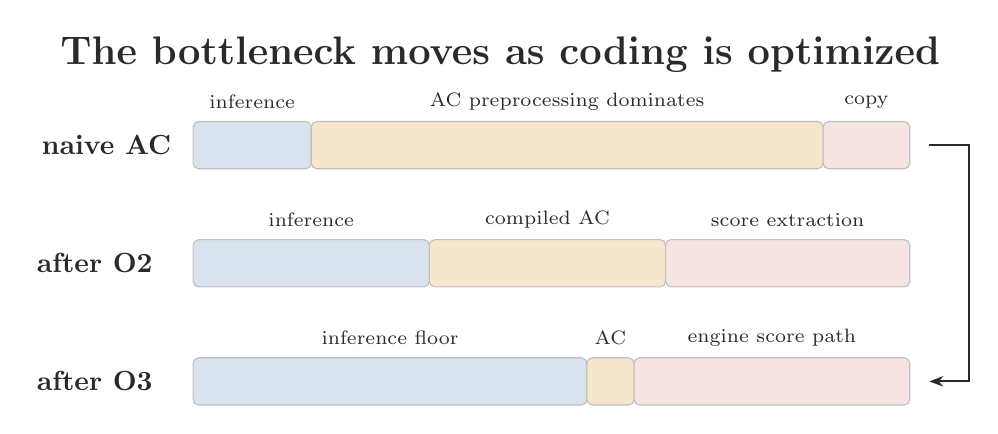
\begin{tikzpicture}[
  x=1cm,y=1cm,
  font=\sffamily,
  bar/.style={draw=ceInk!30, rounded corners=2pt, minimum height=0.62cm},
  lab/.style={font=\scriptsize, ceInk},
  arr/.style={-{Stealth[length=5pt]}, thick, ceInk},
]
  \node[font=\Large\bfseries, ceInk] at (6.4,5.7) {The bottleneck moves as coding is optimized};

  \node[lab, font=\bfseries] at (1.4,4.55) {naive AC};
  \draw[bar, fill=ceBlue!18] (2.5,4.25) rectangle (4.0,4.85);
  \draw[bar, fill=ceGold!25] (4.0,4.25) rectangle (10.5,4.85);
  \draw[bar, fill=ceRed!15] (10.5,4.25) rectangle (11.6,4.85);
  \node[lab] at (3.25,5.1) {inference};
  \node[lab] at (7.25,5.1) {AC preprocessing dominates};
  \node[lab] at (11.05,5.1) {copy};

  \node[lab, font=\bfseries] at (1.25,3.05) {after O2};
  \draw[bar, fill=ceBlue!18] (2.5,2.75) rectangle (5.5,3.35);
  \draw[bar, fill=ceGold!25] (5.5,2.75) rectangle (8.5,3.35);
  \draw[bar, fill=ceRed!15] (8.5,2.75) rectangle (11.6,3.35);
  \node[lab] at (4.0,3.6) {inference};
  \node[lab] at (7.0,3.6) {compiled AC};
  \node[lab] at (10.05,3.6) {score extraction};

  \node[lab, font=\bfseries] at (1.25,1.55) {after O3};
  \draw[bar, fill=ceBlue!18] (2.5,1.25) rectangle (7.5,1.85);
  \draw[bar, fill=ceGold!25] (7.5,1.25) rectangle (8.1,1.85);
  \draw[bar, fill=ceRed!15] (8.1,1.25) rectangle (11.6,1.85);
  \node[lab] at (5.0,2.1) {inference floor};
  \node[lab] at (7.8,2.1) {AC};
  \node[lab] at (9.85,2.1) {engine score path};
  \draw[arr] (11.85,4.55) -- (12.35,4.55) -- (12.35,1.55) -- (11.85,1.55);
\end{tikzpicture}
\end{document}
